% Bagian Analisis Hasil Percobaan
    
\section*{Analisis Hasil Percobaan}
\indent
Percobaan pada modul 3 ialah percobaan untuk membuat sebuah desain untuk wadah PCB. Tujuan utama dari pembuatan case ini adalah untuk melindungi PCB atau apapun yang ada di dalamnya. Tanpa adanya case yang melindungi komponen di dalamnya, ada kemungkinan komponen itu akan rusak, berdebu, terkena air dan lain lain. Wadah yang  didesain adalah objek 3 dimensi, jadi peserta memerlukan 3d printer untuk mencetak wadah tersebut. Dalam mendesain sebuah 3d peserta harus mempertimbangkan ukuran dan kemampuan dari 3d printer yang dimiliki. Dengan mempertimbangkan hal tersebut desain bisa lebih efektif dan bisa lebih fokus dengan tujuannya, yaitu melindungi komponen yang ada di dalamnya.

\subsection*{Alat dan Software}
\begin{enumerate}
    \item Alat
        \begin{enumerate}[label*=\arabic*.]
            \item Laptop
            \item 3D Printer
        \end{enumerate}
    \item Software
        \begin{enumerate}[label*=\arabic*.]
            \item Autodesk Fusion
            \item Ultimaker Cura
        \end{enumerate}
    \end{enumerate}

\subsection*{Langkah-langkah}
\begin{enumerate}
    \item Desain case 
    \begin{enumerate}[label*=\arabic*.]
        \item Peserta memulai dengan membuka software 3d desain, kemudian itu mengupload file PCB yang nantinya akan dimasukkan ke dalam case.
        \begin{figure}[H]
            \centering
            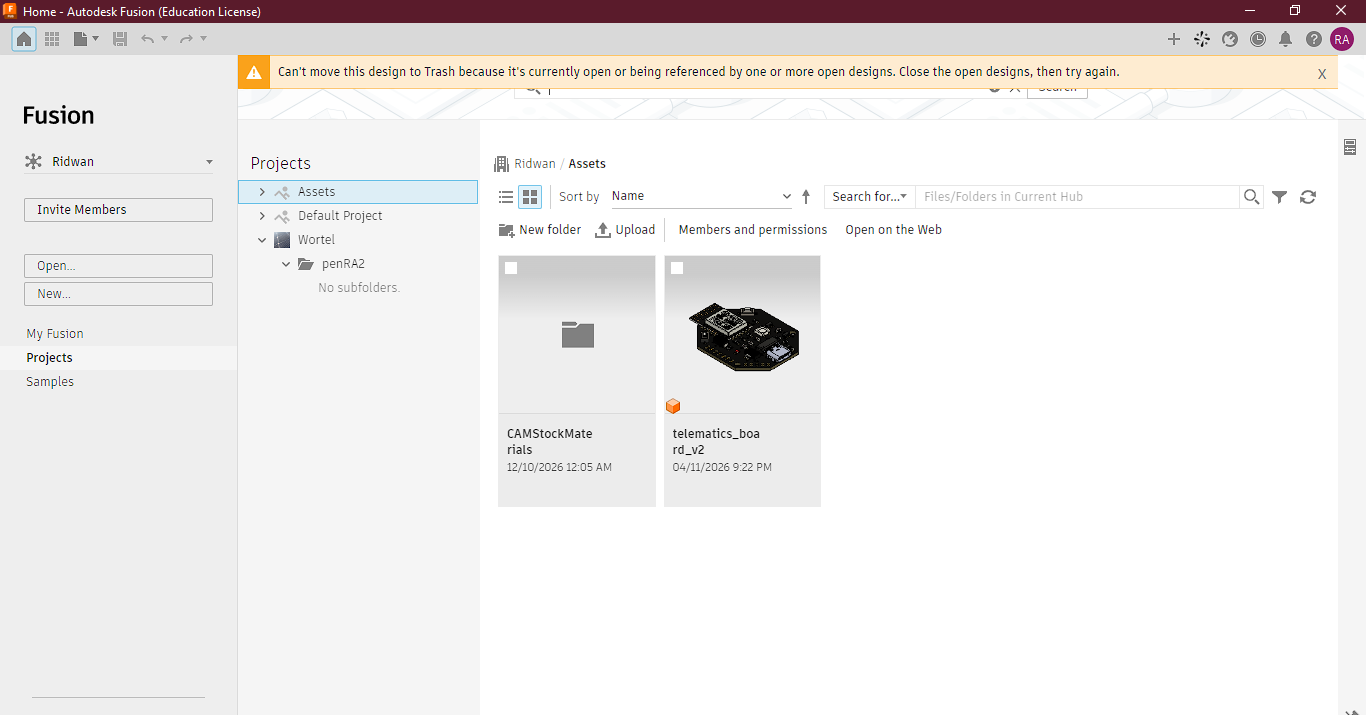
\includegraphics[width=\linewidth]{img/upload.png}
            \caption{Gambar proses upload.}
        \end{figure}
        \item Kemudian peserta membuat sketsa dengan tools sketch dan menggambar desain case yang sesuai dengan ukuran PCB dan membiarkan beberapa area terbuka untuk komponen yang telah ditentukan.
        \begin{figure}[H]
            \centering
            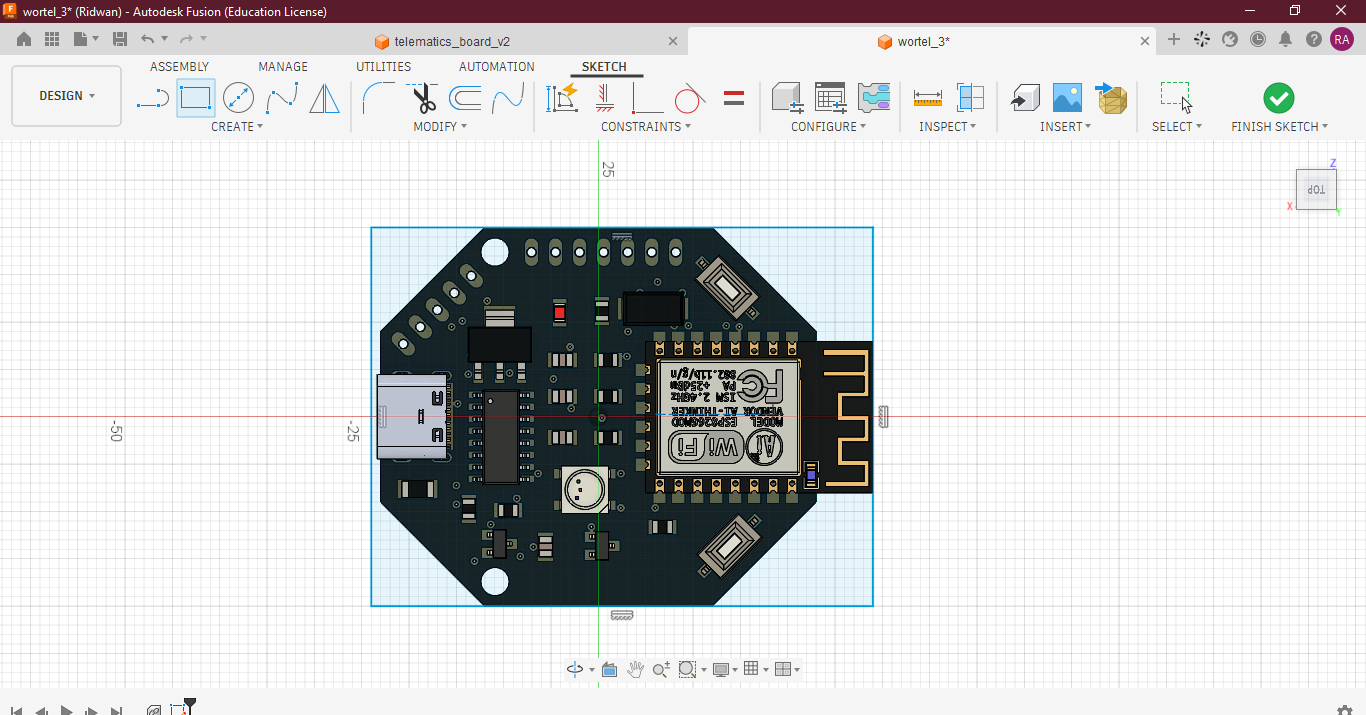
\includegraphics[width=\linewidth]{img/sketch.png}
            \caption{Gambar proses sketch.}
        \end{figure}
        \item Sketsa yang bagian cornernya membentuk siku-siku bisa dibuat melengkung dengan menggunakan tools fillet.
        \item Setelah sketsa selesai, tools extrude digunakan untuk mewujudkan sketsa yang awalnya 2 dimensi menjadi 3 dimensi.
        \begin{figure}[H]
            \centering
            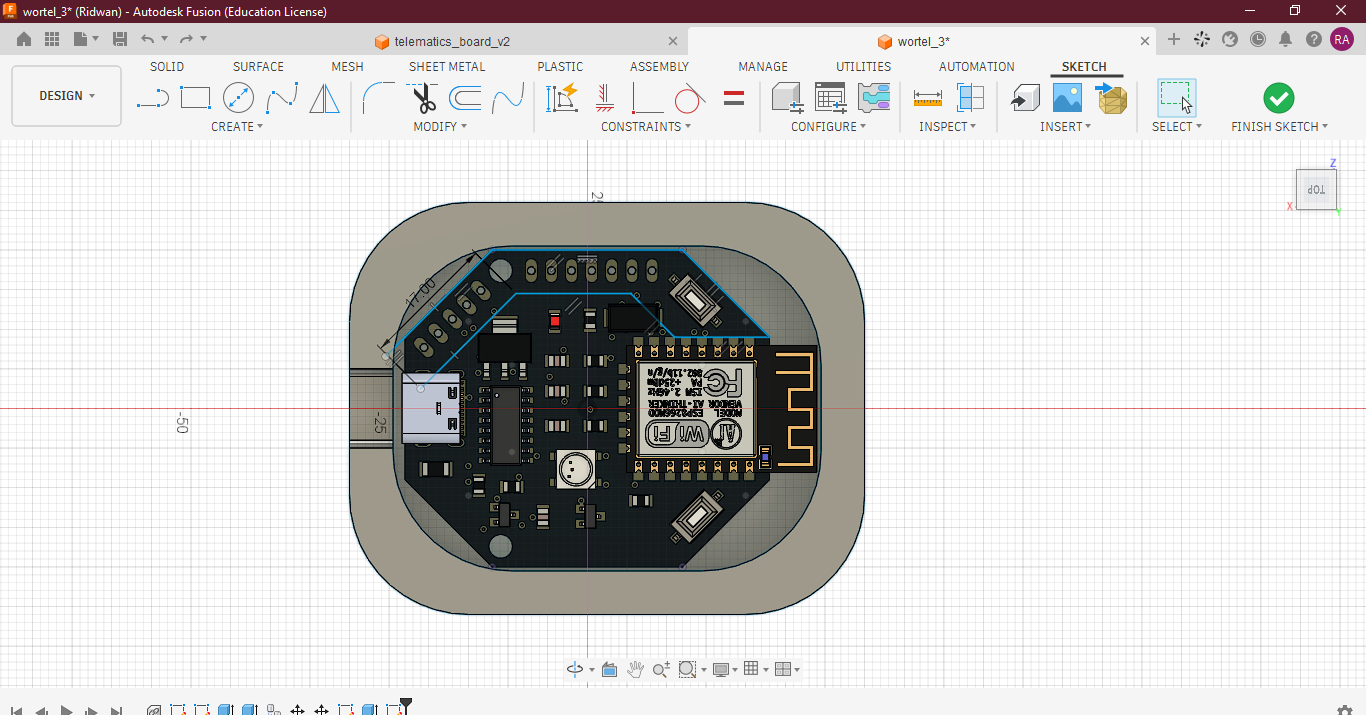
\includegraphics[width=\linewidth]{img/ex.png}
            \caption{Gambar penggunaan extrude.}
        \end{figure}
        \item Selain mewujudkan sketsa menjadi 3 dimensi, tools extrude juga digunakan untuk membuat lubang pada case.
        \item Peserta membuat 2 wujud 3d, yaitu untuk bagian atas dan bagian bawah. Keduanya disesuikan agar bisa ditutup dan dibuka.
        \begin{figure}[H]
            \centering
            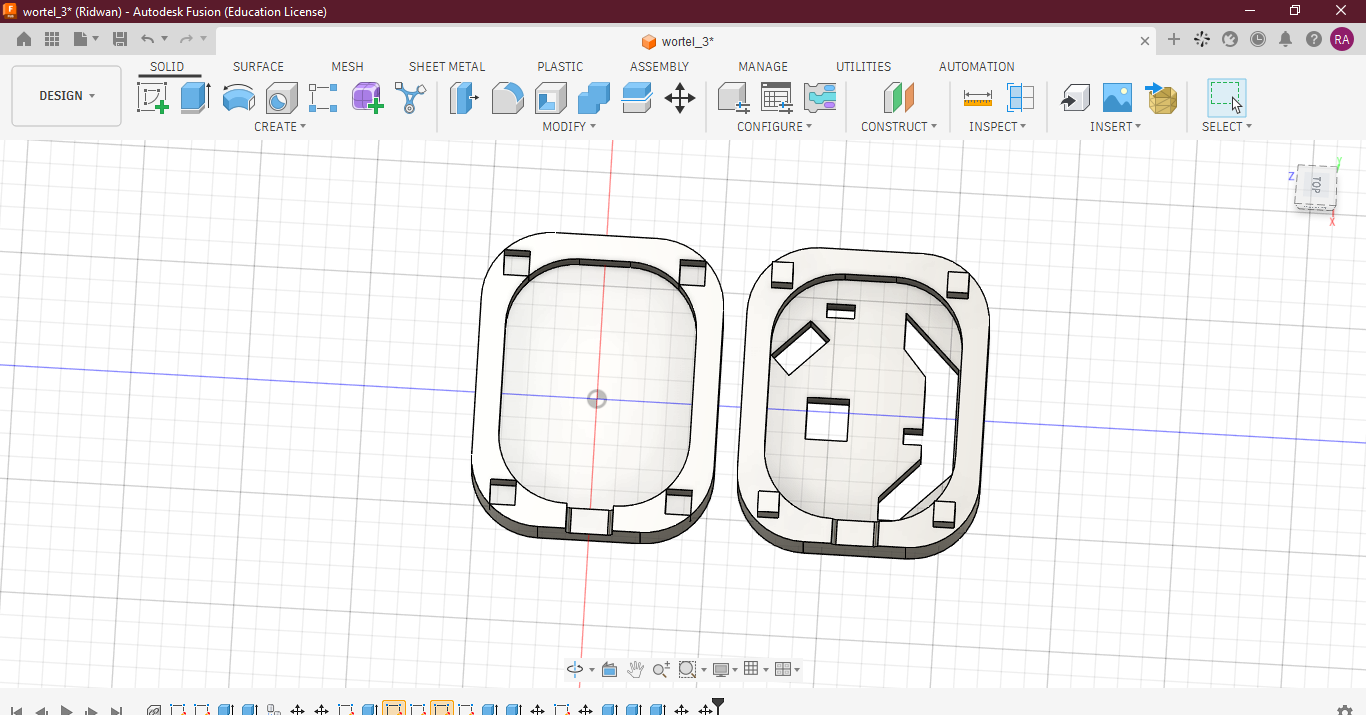
\includegraphics[width=\linewidth]{img/done.png}
            \caption{Gambar Desain Selesai.}
        \end{figure}
    \end{enumerate}
    \item Mencetak case
    \begin{enumerate}[label*=\arabic*.]
        \item Desain yang telah dibuat kemudian diexport menjadi file STL agar bisa dicetak menggunakan 3d Printer.
        \item Kedua file atas dan bawah diatur agar bisa dicetak. Peserta kedunya menghadap ke atas agar bisa dicetak dengan lebih efisien.
        \begin{figure}[H]
            \centering
            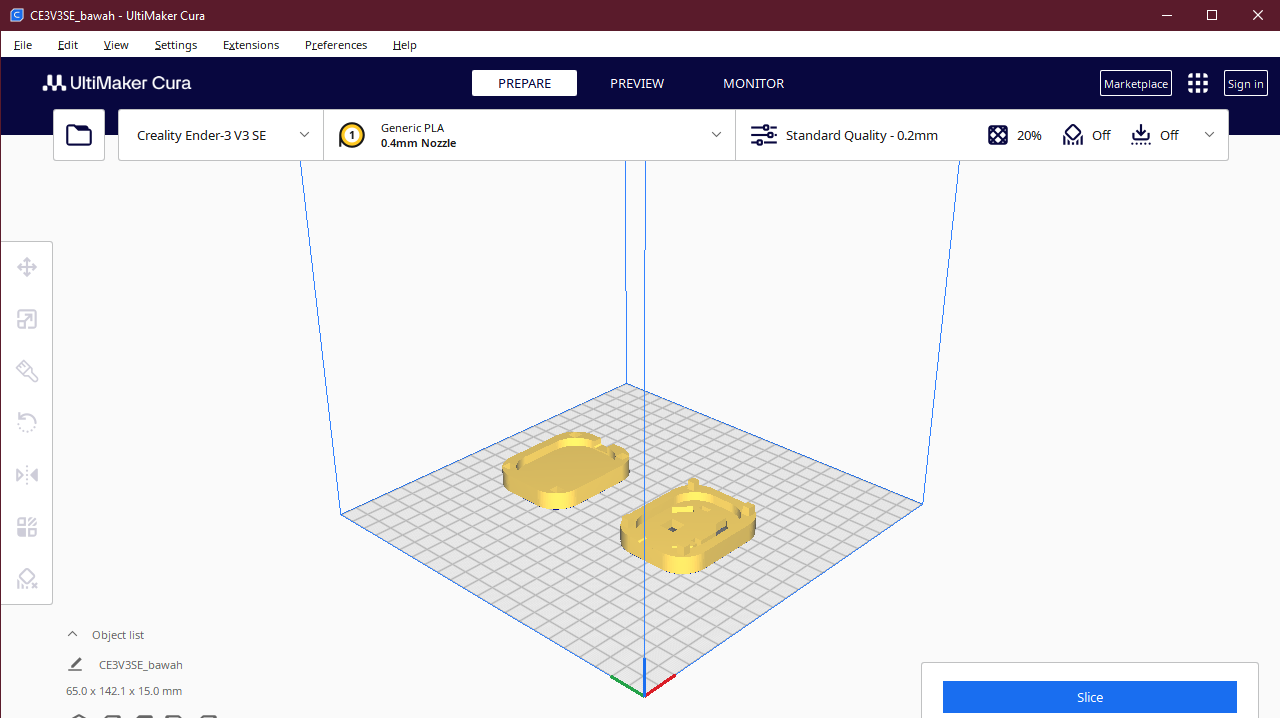
\includegraphics[width=\linewidth]{img/imp.png}
            \caption{Gambar import file ke Cura.}
        \end{figure}
        \item Peserta juga mengatur settingan printer dan mengatur kualitas di Ultimaker Cura agar hasilnya sesuai dengan bahan yang digunakan.
        \begin{figure}[H]
            \centering
            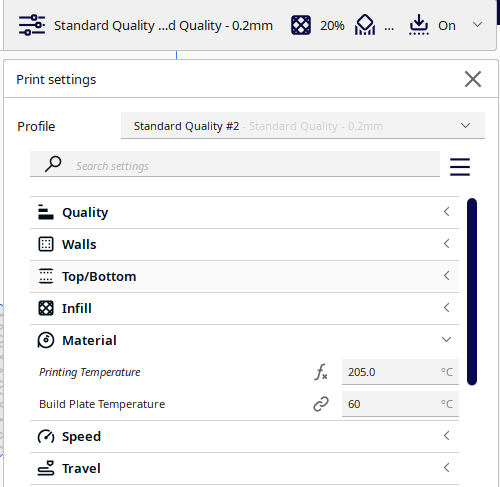
\includegraphics[width=\linewidth]{img/setting.png}
            \caption{Gambar pengaturan printer.}
        \end{figure}
        \item Kemudian peserta bisa melakukan review untuk mengetahui perkiraan hasil cetakannya.
        \item Setelah itu file bisa disimpan dengan format GCODE ke penyimpanan.
    \end{enumerate}
\end{enumerate}

% \begin{table}[h]
%     \centering
%     \caption{Caption tabelnya}
%     \label{tab:labelini}
%     \begin{tabular}{|c|c|c|}
%         \hline
%         Kolom 1 & Kolom 2 & Kolom 3 \\
%         \hline
%         Data 1 & Data 2 & Data 3 \\
%         Data 4 & Data 5 & Data 6 \\
%         \hline
%     \end{tabular}
% \end{table}